\def \CILKserialbaseline {960.2}
\def \CILKblocksize {64}
\def \CILKnumtrials {5}
\def \CILKinputsize {268435456}
\def \CILKtable {
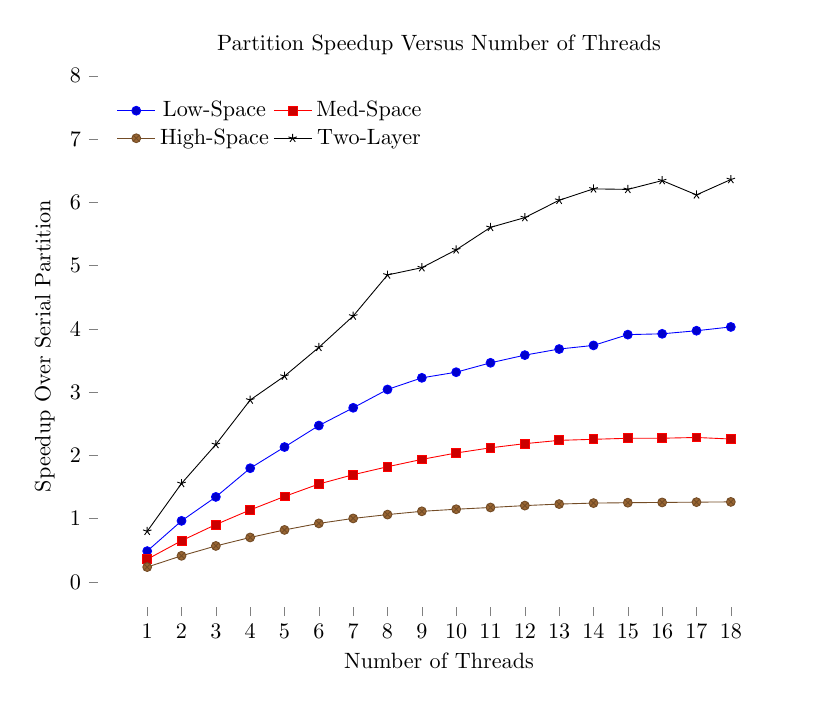
\begin{tikzpicture}[scale = .8]
\begin{axis}[
width = 5in, %%!!!!
height = 4in,
title={Partition Speedup Versus Number of Threads}, %% titles
xtick pos=left,
ytick pos=left,
legend style={draw=none},
axis line style = { draw = none },
legend pos= north west,
xtick = data,
xlabel={Number of Threads},
ylabel={Speedup Over Serial Partition},
ymax = 8,
legend columns = 2,
scatter/classes=%
{a={mark=o,draw=blue}}]
%% In-Place
\addplot coordinates {( 1, 0.487907) ( 2, 0.965802) ( 3, 1.34444) ( 4, 1.79813) ( 5, 2.13283) ( 6, 2.47219) ( 7, 2.75287) ( 8, 3.04246) ( 9, 3.22648) ( 10, 3.31561) ( 11, 3.46392) ( 12, 3.58551) ( 13, 3.68175) ( 14, 3.7391) ( 15, 3.90961) ( 16, 3.92239) ( 17, 3.97105) ( 18, 4.03107) };
%% In-Place Prefix-Sum
\addplot coordinates {( 1, 0.358766) ( 2, 0.651955) ( 3, 0.907905) ( 4, 1.13876) ( 5, 1.35163) ( 6, 1.54821) ( 7, 1.69527) ( 8, 1.82132) ( 9, 1.93745) ( 10, 2.03864) ( 11, 2.12058) ( 12, 2.18625) ( 13, 2.23823) ( 14, 2.25505) ( 15, 2.27105) ( 16, 2.27212) ( 17, 2.28402) ( 18, 2.25929) };
%% Out-of-Place
\addplot coordinates {( 1, 0.235332) ( 2, 0.413416) ( 3, 0.569311) ( 4, 0.703443) ( 5, 0.822512) ( 6, 0.92594) ( 7, 1.00439) ( 8, 1.06523) ( 9, 1.11677) ( 10, 1.14966) ( 11, 1.17729) ( 12, 1.20719) ( 13, 1.23134) ( 14, 1.24669) ( 15, 1.25287) ( 16, 1.25714) ( 17, 1.26176) ( 18, 1.26575) };
%% High-Span
\addplot coordinates {( 1, 0.801099) ( 2, 1.55681)  ( 3, 2.17307)  ( 4, 2.8762) ( 5, 3.25372)  ( 6, 3.70779) ( 7, 4.20367)  ( 8, 4.85267) ( 9, 4.96798)  ( 10, 5.25) ( 11, 5.6049)  ( 12, 5.75928) ( 13, 6.03388)  ( 14, 6.21318)( 15, 6.20516)  ( 16, 6.34433) ( 17, 6.11832)  ( 18, 6.36111) };
\legend{Low-Space, Med-Space, High-Space, Two-Layer}
\end{axis}
\end{tikzpicture}
}
\def \cilktwoblocksizetwo {64}
\def \cilktwonumtrialstwo {5}
\def \cilktwonumcorestwo {18}
\def \cilktwoinputsizetwo {268435456}
\def \cilktwotabletwo {
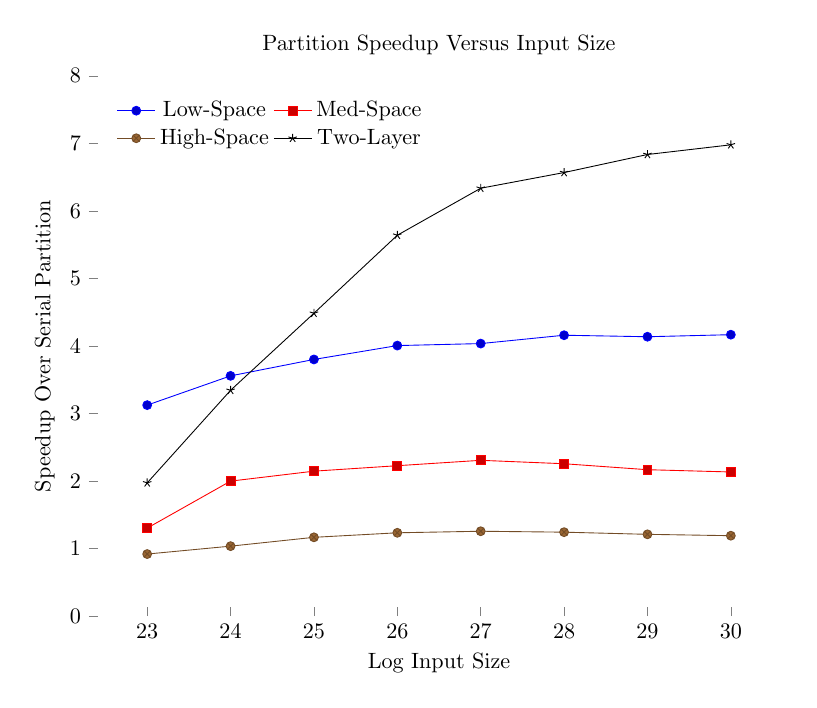
\begin{tikzpicture}[scale = .8]
\begin{axis}[
width = 5in, %%!!!!
height = 4in,
title={Partition Speedup Versus Input Size},
xtick pos=left,
ytick pos=left,
legend style={draw=none},
axis line style = { draw = none },
legend pos= north west,
xtick = data,
xlabel={Log Input Size},
ylabel={Speedup Over Serial Partition},
ymax = 8, %!!!
ymin = 0,
legend columns = 2,
scatter/classes=%
{a={mark=o,draw=blue}}]
%% baselines in ms: \addplot coordinates {( 23, 30 ) ( 24, 61.2 ) ( 25, 122.4 ) ( 26, 246 ) ( 27, 491.6 ) ( 28, 979.2 ) ( 29, 1950.4 ) ( 30, 3909.4 ) };
%% In-Place
\addplot coordinates {( 23, 3.125) ( 24, 3.55814) ( 25, 3.80124) ( 26, 4.00651) ( 27, 4.03612) ( 28, 4.15973) ( 29, 4.13746) ( 30, 4.1678) };
%% In-Place Prefix-Sum
\addplot coordinates {( 23, 1.30435) ( 24, 2) ( 25, 2.14737) ( 26, 2.22826) ( 27, 2.30798) ( 28, 2.25726) ( 29, 2.16904) ( 30, 2.13535) };
%% Out-of-Place
\addplot coordinates {( 23, 0.920245) ( 24, 1.03729) ( 25, 1.16794) ( 26, 1.23494) ( 27, 1.25793) ( 28, 1.24422) ( 29, 1.21218) ( 30, 1.19204) };
%% High-Span
\addplot coordinates {( 23, 1.97368) ( 24, 3.34444) ( 25, 4.48507) ( 26, 5.64019) ( 27, 6.33596) ( 28, 6.56812) ( 29, 6.83522) ( 30, 6.97867) };
\legend{Low-Space, Med-Space, High-Space, Two-Layer}
\end{axis}
\end{tikzpicture}
}
\def \CILKsortblocksize {64}
\def \CILKsortnumtrials {5}
\def \CILKsortmaxinputsize {268435456}
\def \CILKsorttable {
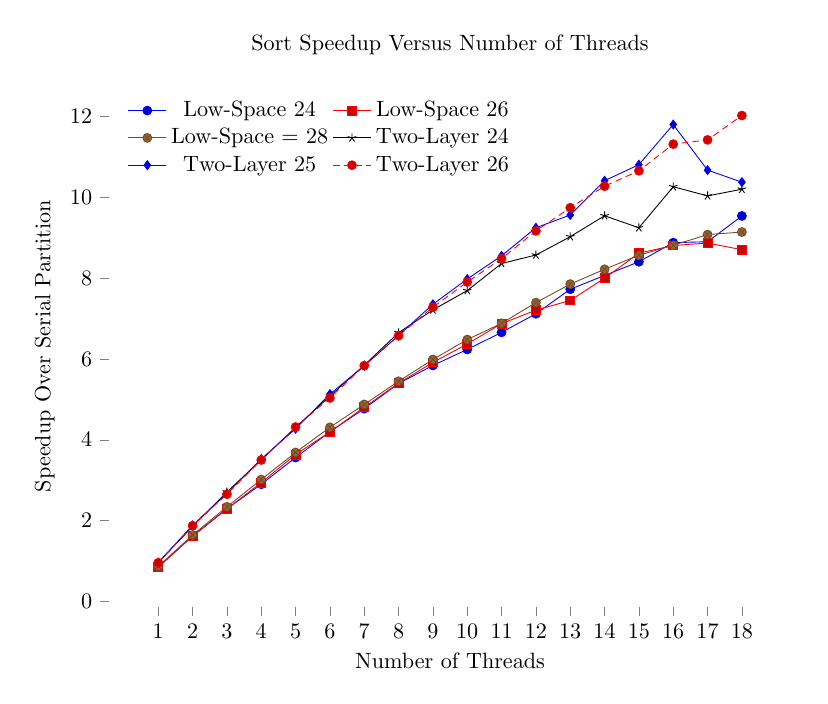
\begin{tikzpicture}[scale = .8]
\begin{axis}[
width = 5in, %%!!!!
height = 4in,
title={Sort Speedup Versus Number of Threads},
xtick pos=left,
ytick pos=left,
legend style={draw=none},
axis line style = { draw = none },
legend pos= north west,
xtick = data,
xlabel={Number of Threads},
ylabel={Speedup Over Serial Partition},
ymax = 13,
legend columns = 2,
scatter/classes=%
{a={mark=o,draw=blue}}]
\addplot coordinates {( 1, 0.851926) ( 2, 1.61836) ( 3, 2.29358) ( 4, 2.90128) ( 5, 3.56004) ( 6, 4.19852) ( 7, 4.77091) ( 8, 5.39237) ( 9, 5.83749) ( 10, 6.23416) ( 11, 6.65588) ( 12, 7.11635) ( 13, 7.72355) ( 14, 8.06295) ( 15, 8.40223) ( 16, 8.87451) ( 17, 8.89777) ( 18, 9.53511) };
\addplot coordinates {( 1, 0.853455) ( 2, 1.61249) ( 3, 2.29409) ( 4, 2.94183) ( 5, 3.63486) ( 6, 4.19491) ( 7, 4.80463) ( 8, 5.39938) ( 9, 5.91257) ( 10, 6.36984) ( 11, 6.87319) ( 12, 7.20401) ( 13, 7.44596) ( 14, 7.99512) ( 15, 8.61408) ( 16, 8.80442) ( 17, 8.8653) ( 18, 8.7005) };
\addplot coordinates {( 1, 0.86917) ( 2, 1.64562) ( 3, 2.34338) ( 4, 3.01686) ( 5, 3.68602) ( 6, 4.30734) ( 7, 4.87436) ( 8, 5.44601) ( 9, 5.98517) ( 10, 6.4772) ( 11, 6.88037) ( 12, 7.39233) ( 13, 7.849) ( 14, 8.21602) ( 15, 8.56351) ( 16, 8.81014) ( 17, 9.07398) ( 18, 9.13702) };
\addplot coordinates {( 1, 0.96519) ( 2, 1.85909) ( 3, 2.70997) ( 4, 3.50154) ( 5, 4.30891) ( 6, 5.07893) ( 7, 5.8449) ( 8, 6.64815) ( 9, 7.21036) ( 10, 7.68997) ( 11, 8.35907) ( 12, 8.5691) ( 13, 9.02249) ( 14, 9.53986) ( 15, 9.24255) ( 16, 10.2571) ( 17, 10.0309) ( 18, 10.1958) };
%% High-Span with log size 26
\addplot coordinates {( 1, 0.96416) ( 2, 1.88464) ( 3, 2.67182) ( 4, 3.52606) ( 5, 4.274) ( 6, 5.12953) ( 7, 5.8281) ( 8, 6.58099) ( 9, 7.35149) ( 10, 7.9753) ( 11, 8.54922) ( 12, 9.2437) ( 13, 9.55906) ( 14, 10.4064) ( 15, 10.8039) ( 16, 11.7951) ( 17, 10.6681) ( 18, 10.3701) };
%% High-Span with log size 28
\addplot coordinates {( 1, 0.959398) ( 2, 1.87539) ( 3, 2.65486) ( 4, 3.50039) ( 5, 4.31537) ( 6, 5.03388) ( 7, 5.83344) ( 8, 6.5715) ( 9, 7.27783) ( 10, 7.90044) ( 11, 8.47848) ( 12, 9.16563) ( 13, 9.73822) ( 14, 10.2711) ( 15, 10.6513) ( 16, 11.3112) ( 17, 11.416) ( 18, 12.0183) };
\legend{Low-Space 24, Low-Space 26, Low-Space = 28, Two-Layer 24, Two-Layer 25, Two-Layer 26}
\end{axis}
\end{tikzpicture}
}
\def \partitionbandwidthboundserialbaseline {982.4}
\def \partitionbandwidthboundblocksize {64}
\def \partitionbandwidthboundnumtrials {5}
\def \partitionbandwidthboundinputsize {268435456}
\def \partitionbandwidthboundtable {
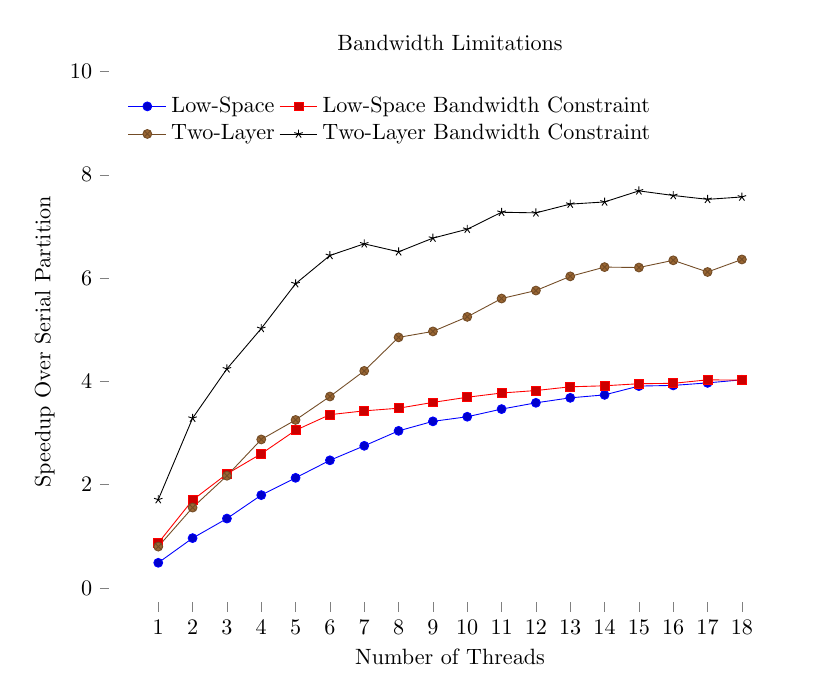
\begin{tikzpicture}[scale = .8]
\begin{axis}[
width = 5in, %%!!!!
height = 4in,
title={Bandwidth Limitations},
xtick pos=left,
ytick pos=left,
legend style={draw=none},
axis line style = { draw = none },
legend pos= north west,
xtick = data,
xlabel={Number of Threads},
ylabel={Speedup Over Serial Partition},
ymax = 10,
legend columns = 2,
scatter/classes=%
{a={mark=o,draw=blue}}]
\addplot coordinates {( 1, 0.487907) ( 2, 0.965802) ( 3, 1.34444) ( 4, 1.79813) ( 5, 2.13283) ( 6, 2.47219) ( 7, 2.75287) ( 8, 3.04246) ( 9, 3.22648) ( 10, 3.31561) ( 11, 3.46392) ( 12, 3.58551) ( 13, 3.68175) ( 14, 3.7391) ( 15, 3.90961) ( 16, 3.92239) ( 17, 3.97105) ( 18, 4.03107) };
\addplot coordinates {(1, 0.871473)(2, 1.70224)(3, 2.20891)(4, 2.59909)(5, 3.05396)(6, 3.35607)(7, 3.42998)(8, 3.48084)(9, 3.59341)(10, 3.69352)(11, 3.7752)(12, 3.82343)(13, 3.89536)(14, 3.9152)(15, 3.95524)(16, 3.96281)(17, 4.03066)(18, 4.02384)};
%% High-Span Bandwidth Bound
\addplot coordinates {( 1, 0.801099) ( 2, 1.55681)  ( 3, 2.17307)  ( 4, 2.8762) ( 5, 3.25372)  ( 6, 3.70779) ( 7, 4.20367)  ( 8, 4.85267) ( 9, 4.96798)  ( 10, 5.25) ( 11, 5.6049)  ( 12, 5.75928) ( 13, 6.03388)  ( 14, 6.21318)( 15, 6.20516)  ( 16, 6.34433) ( 17, 6.11832)  ( 18, 6.36111) };
\addplot coordinates {(1, 1.71059)(2, 3.288)(3, 4.24304)(4, 5.02466)(5, 5.89179)(6, 6.4389)(7, 6.66406)(8, 6.50981)(9, 6.77436)(10, 6.94659)(11, 7.27545)(12, 7.26331)(13, 7.4328)(14, 7.47498)(15, 7.68927)(16, 7.59996)(17, 7.52513)(18, 7.57127)};
\legend{Low-Space, Low-Space Bandwidth Constraint, Two-Layer, Two-Layer Bandwidth Constraint} %% !!!
\end{axis}
\end{tikzpicture}
}
